\section{Abgrenzung des Projektes}
In diesem Kapitel soll eine Abgrenzung des Projektes gegenüber anderen bereits vorhandenen Lösungen und dem späteren vollständig ausgebildeten Güterwagen 4.0 stattfinden. \par
\begin{figure}[hbp]
    \centering
    \definecolor{red1}{RGB}{228,26,28}
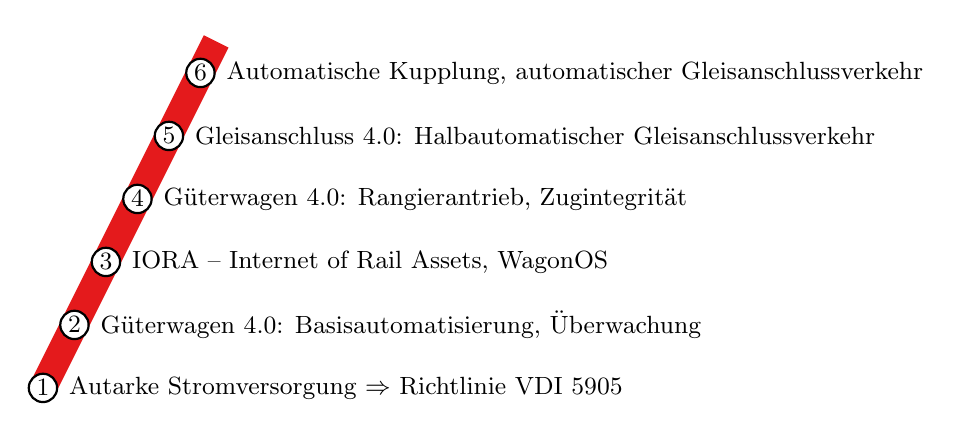
\begin{tikzpicture}[font = \sffamily, scale = 0.8]
\tikzstyle{every node}=[font=\small]
\path[line width = .35cm, draw = red1] (0,0) -- (2.75,5.5);
\path[draw, thick, fill = white] (0,0) node[circle, draw, fill = white, inner sep = 1] {1}  node[xshift = .2cm, anchor = west] {Autarke Stromversorgung $\Rightarrow$ Richtlinie VDI 5905};

\path[draw, thick, fill = white] (0.5,1) node[circle, draw, fill = white, inner sep = 1] {2} node[xshift = .2cm, anchor = west] {Güterwagen 4.0: Basisautomatisierung, Überwachung};

\path[draw, thick, fill = white] (1,2) node[circle, draw, fill = white, inner sep = 1] {3}  node[xshift = .2cm, anchor = west] {IORA -- Internet of Rail Assets, WagonOS};

\path[draw, thick, fill = white] (1.5,3) node[circle, draw, fill = white, inner sep = 1] {4} node[xshift = .2cm, anchor = west] {Güterwagen 4.0: Rangierantrieb, Zugintegrität};

\path[draw, thick, fill = white] (2,4) node[circle, draw, fill = white, inner sep = 1] {5}  node[xshift = .2cm, anchor = west] {Gleisanschluss 4.0: Halbautomatischer Gleisanschlussverkehr};

\path[draw, thick, fill = white] (2.5,5) node[circle, draw, fill = white, inner sep = 1] {6}  node[xshift = .2cm, anchor = west] {Automatische Kupplung, automatischer Gleisanschlussverkehr};
\end{tikzpicture}
    \caption{Railmap [QUELLE]}
    \label{fig:Railmap}
\end{figure}
Bereits in diversen Vorträgen [QUELLE] kam es zur Vorstellung der sogenannten Railmap, siehe dazu auch Abbildung \ref{fig:Railmap}, diese Zeit den Plan für zukünftige Entwicklungen im Schienengüterverkehr. Auf dieser ist der Weg abgebildet, den unter anderem auch der Güterwagen 4.0  gehen soll, aber auch weitere Punkte, die danach für die Automatisierung des Schienengüterverkehrs folgen sollen. Die Railmap beginnt mit dem Hauptpunkt, der auch ein Schwerpunkt dieses Projektes sein soll, der autarken Stromversorgung des Wagens.\par
Der zweite Punkt der Railmap besteht dann aus dem vollständigen Güterwagen (siehe dazu auch Kapitel \ref{sec:Ausbaustufen} mit Automatisierung verschiedener Systeme, Überwachung von einzelnen Subsystemen und einem Rangierantrieb. In diesem Projekt soll eine Ausrüstung des Wagens bis Ausbausstufe 3 erfolgen. Ein Ausbau der Klassen 4 und 5 ist nicht geplant. \par
Im dritten Punkt ist dann bereits eine dezentrale, unabhängige Intelligenz von Güterwagen geplant. Diese soll dem Internet of Things entsprechen. Dem Internet of Rail Assets. In diesem Punkt soll es für den Güterwagen möglich sein mit anderen 'Dingen' der Eisenbahn zu kommunizieren.\par
Im vierten Punkt geht es bereits um halbautomatiserten Gleisanschlussverkehr und den sogeannten Gleisanschluss 4.0. auch hierzu gibt es bereits vorgestellte Ideen. Zum Beispiel auf der 1. BME-VDV-Gleisanschluss-Konferenz. \par
Im fünften und letzten Punkt dieser Railmap soll die automatische Kupplung flächendeckend eingeführt sein und ein automatischer Gleisanschlussverkehr möglich sein.\par
In diesem Projekt soll der Güterwagen ein konventioneller Güterwagen mit konventionellen Fahrwerken und Luftbremse bleiben. Einzig ein zusätzlicher Aufbau von Leistungs- und sicherheitsgerichteten Komponenten ist geplant.\par
\subsection{Leistungsniveau und Energieversorgung}
Diese Stromversorgung soll in diesem Projekt nur für ein geringes Leistungsniveau bereitstehen. Es ist keine Anwendung mit größerer Stromzufuhr geplant. Ein später folgender Güterwagen 4.0  kann dies aber eventuell fordern.\par
In diesem Projekt wird weder die Energieversorgung des späteren 'vollständig' ausgebauten Güterwagen 4.0 noch die Energieversorgung nach der VDI-Richtlinie 5905 entwickelt. Dabei wird es wahrscheinlich Überschneidungen geben, auch werden Erfahrungen aus den Arbeitsrunden mitgenommen und einfließen, aber es wird keine exemplarische Realisierung dessen.\par
\subsection{VDI 5905}
Eine vollständige Stromversorgung nach der VDI-Richtlinie 5905 oder ein Prototyp der diese Richtlinie prägen soll, soll nicht entstehen. 
\subsection{ep-light}
Während dieses Projektes ist eine Ausstattung der Wagen mit einer ep-light-Bremse als Versuch geplant.Diese wird allerdings ohne Anrechnung auf die Bremsleistung im Testbetrieb stattfinden, sodass eine erste Einführung probehalber unkritisch ist. Eine angerechnete ep-Bremse im Güterverkehr wäre aus vielen gründen sehr interessant (SIEHE AUCH), muss allerdings weitreichende geplant sein.\par
\subsection{Labormuster und Demonstrator}
Beim Aufbau ist wichtig, dass sowohl Labormuster als auch Demonstrator nicht später als vollständige Güterwagen 4.0 nutzbar sein werden. Außerdem ist es möglich, dass ein Umbau an der Bremse die Zulassung des Wagens so sehr einschränkt, dass keine Fahrten auf freier Strecke möglich sind. Darum ist darüber zu diskutieren, ob nur ein Erprobungsträger mit automatischer Bremse auszustatten ist, aber eventuell eine dritte (tragbare) Kommunikationsbasis zu erstellen ist, die während einer Erprobung auf freier Strecke auf einen weiteren Wagen zu Testzwecken gesetzt werden kann.\par
Hier folgt weiter eine Abgrenzung zwischen Möglichkeiten, die für den Güterwagen 4.0  mögich sind, und dem Demonstrator anhand von Punkten aus dem Ist-Prozess.
\subsubsection{Beladung und Ladungssicherung}
Hier ist es möglich diverse Sensoren, auch unabhängig von der Beladung mit palletiertem Gut, für Komponenten der Ladungssicherung zu entwickeln und zu überwachen. Beispiele dafür sind:
\begin{itemize}
    \item Königszapfen
    \item Ladeverstellung bei der Automobilverladung
    \item Tragzapfenverstellung bei Containertragwagen
    \item Coiltransporter ?
    \item Verstellbare und verschließbare Trennwände bei Schiebewandwagen
    \item Technische Überwachung von diversen Hebeln und Schaltern
    \itemm Temperatursensoren an temperaturempfindlichem Gut.
    \item ...
\end{itemize}
Auch möglich ist es Spanngurte mit Sensoren in den Textilien zu entwickeln, die über Funkverbindung mit dem Wagen kommunizieren können.\par
Diese Sensoren können mittels Funkkommunikation oder mittels Datenleitung ausgelesen werden. Hier ist auf eine sichere Übertragung zu achten\par
Ebenfalls Vorstellbar sind auch Warnlichter bei Bewegungen des Güterwanges oder eine Alarmanlage.
\subsubsection{Bremse}
Stillstandsüberwachung - Warnlichter - Rundumlicht (Hat auf Werksgelände sonst alles (ist das so? Joachim fragen) oder/und Akustik
Warnfunktion an der Spitze beim Rangieren + Kamera für Unimogfahrer? Fahrer eines Zwei-Wege-Fahrzeuges auf LKW-Basis
Automatische Notbremsfunktion - Handbremse anlegen bei Hindernis - Vorstellbar, aber Standardausrüstung? Wirtschaftliche Betrachtung


\subsection{Beschreibung der Ausbaustufen}\label{sec:Ausbaustufen}
Anhand des Ist- und Soll-Zustandes (siehe folgendes Kapitel) sind fünf Ausbaustufen für den Güterwagen 4.0 geplant, die diese Zeiteinsparung bringen sollen. In den folgenden Abschnitten werden die geplanten Ausbaustufen kurz beschrieben.\par
Die ersten drei Ausbaustufen sollen in diesem Projekt stattfinden. Ausbaustufe 4 und 5 in Folgeprojekten. Eine Zulassung soll über mindestens gleichbleibende Sicherheit bei kompletter Abschaltung des Systems stattfinden. Diese in Schritten stattfindende Automatisierung führt zu einem hohen Mehrwert des Güterwagens, nicht nur, im Einzelwagenverkehr.
\subsubsection{Ausbaustufe 1: Stromversorgung, Telematik und Datenvernetzung}
\begin{figure}[hbp] 
    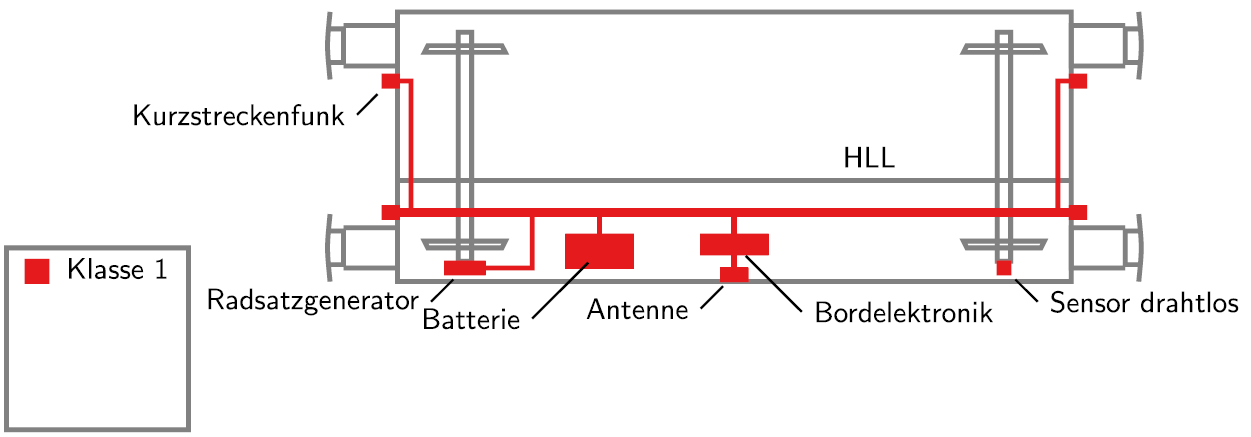
\includegraphics[width=\textwidth]{Bilder/Ausbaustufen_1.PNG}
    \caption{Klasse 1 mit Stromversorgung, Telematik und Datenvernetzung - angelehnt an \cite{ETR_3} }
    \label{fig:Klasse1}
\end{figure} 
In der ersten Ausbaustufe, siehe Abbildung \ref{fig:Klasse1}, ist die Anbringung einer Bordelektronik mit  entsprechender Spannungsversorgung geplant. Die Spannungsversorgung kann als Batterie mit Speisung durch einen Radsatzgenerator, Solarpanels oder ähnlichem realisiert werden oder auch als Pufferbatterie mit Speisung durch AK. Dazu kommen verschiedene Antennen und Kurzstreckenfunk zur Kommunikation mit anderen Wagen. Auch Sensoren zur Erfassung verschiedener Telematikfunktionen sind geplant.\par
In diesem Stadium ist der Wagen an sich noch nicht 'schlauer' als ein nicht ausgerüsteter Wagen, aber er kann sich mitteilen. Mitteilungen könne sein: Standort, Belandung, Laufleistung, (ungewöhnliche) Vibrationen (beispielsweise durch Falschstellen), Heißläuferdedektion, letzte Wartungsintervalle, Zustand der Bremse und vieles mehr.\par
\subsubsection{Ausbaustufe 2: Ausbaustufe 1 + Automatisierung der Bremsbedienung}
\begin{figure}[htbp] 
    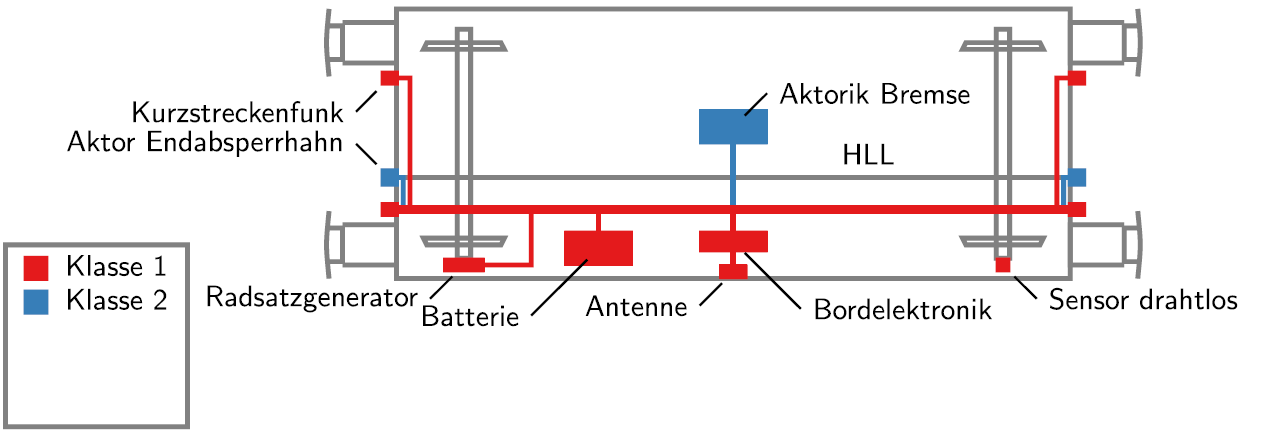
\includegraphics[width=\textwidth]{Bilder/Ausbaustufen_2.PNG}
    \caption{Klasse 2 bestehend aus Klasse 1 und der Automatisierung der Bremsbedienung - angelehnt an \cite{ETR_3}}
    \label{fig:Klasse2}
\end{figure} 
In der zweiten Ausbaustufe ist eine zusätzliche Aktorik für Endabsperrhähne und Handbremse geplant. Dadurch kann ein Teil der Bremsbedienung so weit automatisiert werden, dass ein Einstellen der Bremsart anhand von anderen Wagen im Wagenzug, Gewicht und Bremsfähigkeit möglich ist. Außerdem ist die automatische Parkbremse realisiert.\par
\subsubsection{Ausbaustufe 3: Ausbaustufe 2 + ep-''light''-Bremsen}
\begin{figure}[htbp] 
    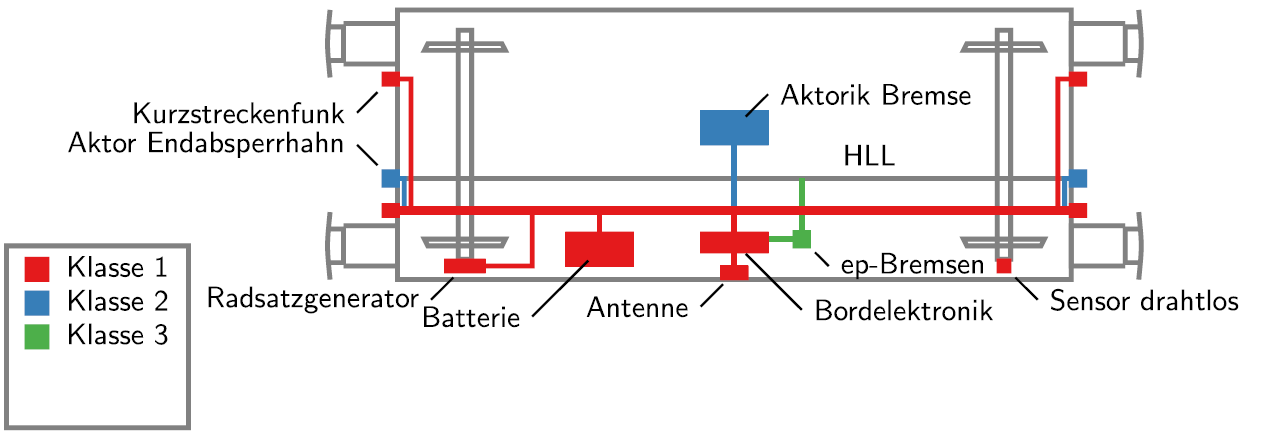
\includegraphics[width=\textwidth]{Bilder/Ausbaustufen_3.PNG}
    \caption{Klasse 3 bestehend aus Klasse 2 und der eingeführten ep-''light'-Bremse - angelehnt an \cite{ETR_3}}
    \label{fig:Klasse3}
\end{figure} 
In der dritten Ausbaustufe kommt zusätzlich zur Bremsbedienung auch die Ep-''light''-Bremse hinzu. Diese sorgt für eine für kürzere Bremswege und/oder höhere Geschwindigkeiten.\par
\subsubsection{Ausbaustufe 4: Ausbaustufe 3 + automatisierter Zugschluss}
\begin{figure}[htbp] 
    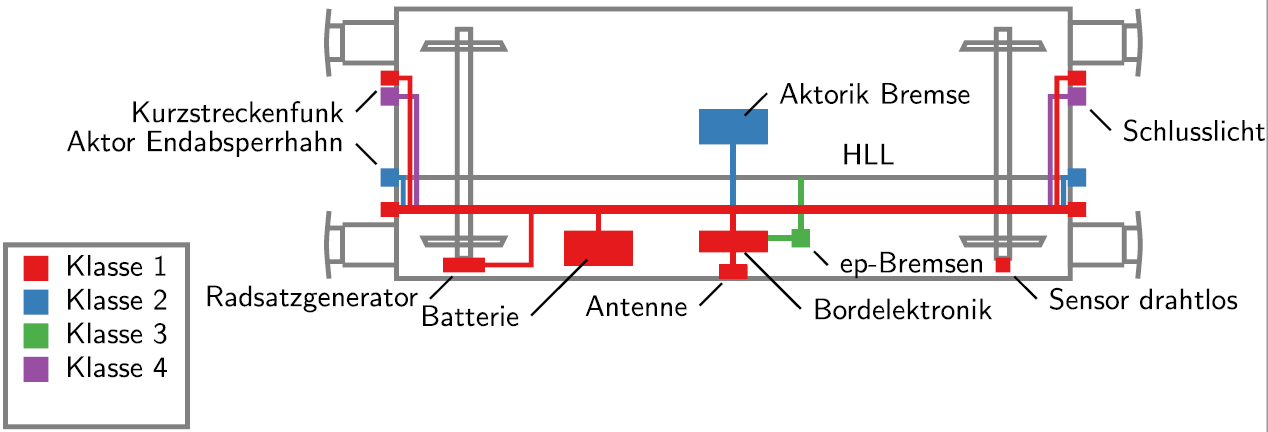
\includegraphics[width=\textwidth]{Bilder/Ausbaustufen_4.PNG}
    \caption{Klasse 4 bestehend aus Klasse 3 und der Automatisierung des Zugschlusses - angelehnt an \cite{ETR_3}}
    \label{fig:Klasse4}
\end{figure} 
In der vierten Ausbaustufe ist ein automatisierter Zugschluss geplant. Dieser soll das Anbringen des Zugschlusssignals am letzten Wagen ablösen. Dies wird eventuell vom Personal noch Manuell erledigt. Dau muss die Person den gesamten Zug von bis zu 700m ablaufen um die die entsprechenden Signale am letzten Wagen anzubringen. Das Zugschlusssignal hat außerdem die Funktion die Zugintigrität zu gewährleisten. 
\subsubsection{Ausbaustufe 5: Ausbaustufe 4 + Rangierantrieb}
\begin{figure}[htbp] 
    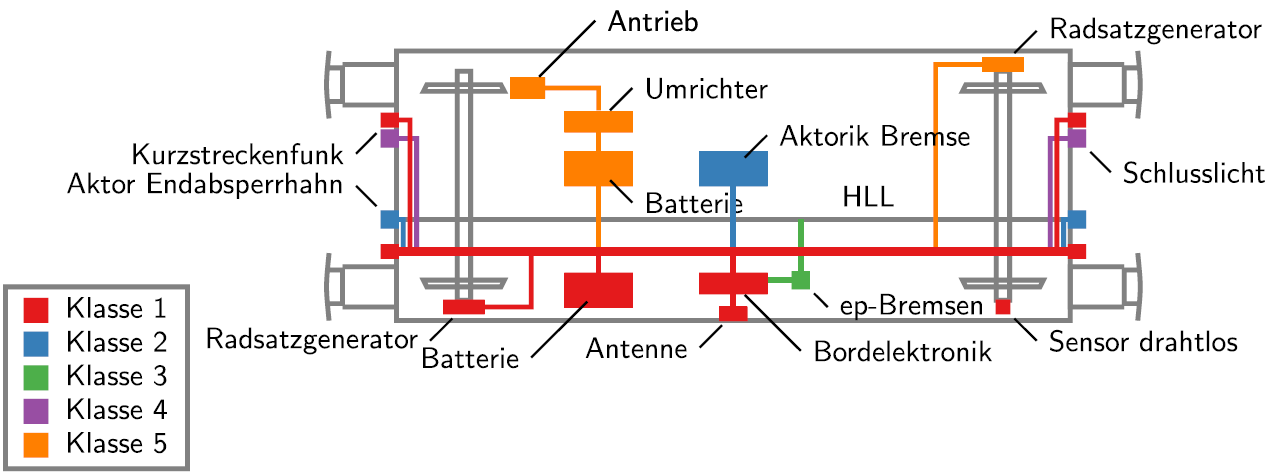
\includegraphics[width=\textwidth]{Bilder/Ausbaustufen_5.PNG}
    \caption{Klasse 5 bestehend aus Klasse 4 und einem Rangierantrieb - angelehnt an \cite{ETR_3}}
    \label{fig:Klasse5}
\end{figure} 
In der fünften Ausbaustufe kommt der Rangierantrieb hinzu. Damit dieser ohne Probleme funktioniert brauch er neben einem Antrieb zusätzlich eine weitere Batterie und Umrichter. Zur Speisung der zweiten Batterie wird auch ein zweiter Radsatzgenerator benötigt.\par
In diesem Stadium kann von einem automatisierten Güterwagen gesprochen werden. Er kann selbstständig bei der ''Briefkastenbedienung'' assistieren und auf dem Werksgelände ohne Rangierlok verfahren.
